\section{Methods}
\subsection{Dataset}
The dataset is data collected from the Children’s Hospital Boston, consisting in EEG recordings of subjects with intractable seizures. The folders classify in 23 cases from 22 subjects (case chb21 and chb1 are the same but 1.5 years apart). The subject’s personal information gender and age is in a separate file called SUBJECT-INFO added in this paper as subject\_info.csv.
\\\\
Each case contains between 9 and 42 .edf files. There are .edf files of EEG signals without seizures and others with recordings of seizures, these defined in RECORDS-WITH-SEIZURES. The files with seizures have the extension .edf.seizures which disables the possibility of accessing the file with a normal edf reader library.
\\\\
Most cases have 1 hour of EEG recordings, but some have 1 to 4 hours depending on the case, split between 9 to 42 edf recordings, recorded at 256Hz in 16 bit resolution. It’s important to note, some subjects had hardware interruptions while the recording of the EEG, and so when there is an interruption, it’s noted in the summary.txt file. This kind of interruptions are a problem to get information normally, because the disposition of the electrodes change making it harder to take in to account the disposition of the electrodes and the EEG doesn’t work for a sequential approach, for example, if it’s important there is hypothetically an order on how a seizure comes to be, this file would certainly be discarded. To take into account this file the script to process the data in this TFG should be programmed to do so. For now, the objective is different, this project just classifies if there is or not a seizure, but for further development it should be considered. The data base is very large containing enough uninterrupted data to work with.
\\\\
The data used to train the model in this TFG is data from subject 1 to subject 10, because the database I huge and time and resources are limited. Also only few .edf in each subject’s folders have any seizure. If every. edf was used there would be a lot more data labelled as not seizure than seizure data, so from each subject only the files with seizure are used, and from these files data is cut to have a balance of labelled data of 50% data with seizure and 50% data without.
\\\\
The model of the CVC uses numpy array as input to work, and other data filtering is usually done in .parquet format, so this TFG uses mainly these two formats to work with data. Starting by .edf files on the database it’s processed to .parquet format, and once is saved again with this format it’s saved again in .npy.
\\\\
The first script to be executed is ReadEDF.py which gets the raw data from every folder of every subject and filters every .edf from each one. It filters the raw data with the bandwidth desired to work with in the model and stets the labelling of every file. Because of the strategy used in this TFG every subject has an average of 5 .edf files. Each one has 22 different channels, which are the electrodes of the subject. In order to label the data, a new column is created (the 23rd) as seizure with the information of every row being a seizure or not and also a 24th column to set the observation windows for the model.
\\\\
All this information is then saved as stated previously in parquet format to access if needed, furthermore in order for the model to accept data the parquets are split into two numpy arrays, one of data\_x with the number of windows, electrodes and data. Another numpy array data\_y with seizure window, being a dimension of data, which defines if a window has or not a seizure in it, and another dimension defining each window.
\\\\
With this, all the parquets and arrays are specifically saved and ordered to ensure easy access and fast comprehension of the herarchy of folders. The database folder has every subject folder and a folder to save the model if needed ordered in it by the date of execution. In every folder of the subject there are 3 more sorted by edf, parquet and numpy folders.
\\\\

\begin{figure}[h!]
    \caption{Filtered data in Theta range from electrode FP1-F7, subject 1 file 3}
    \centering
    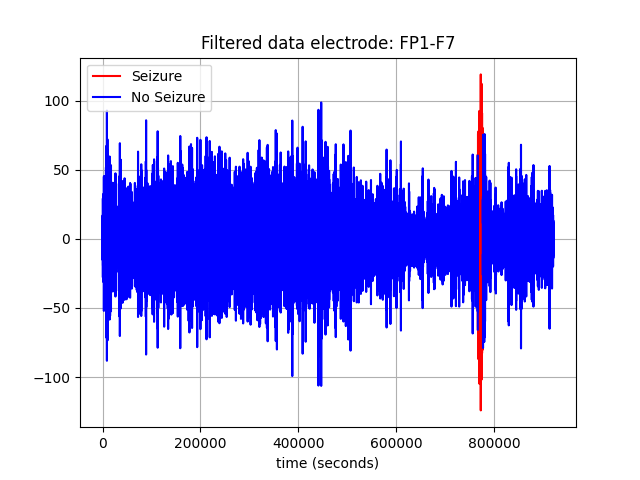
\includegraphics[width=0.5\textwidth]{img/seizurenoseizure.png}
\end{figure}

\leavevmode\\
\subsection{Network}
An already done deep learning algorithm is used from the research group IAM from the CVC, which is working on a framework to determine the optimal architecture for cognitive state recognition from EEG signals, with the objective to answer different questions:
\\
\begin{itemize}
\item How to combine the signals to create the input features for feature extraction? In this case, having 14 sensors x 5 waves, so 70 raw signals. These signals can be concatenated, or projected. As well, in case of projection, the weights can be equal or learned.
\item Which neural network is the best performer?
\item Is it better to ensemble the different classifiers before combining the signals?
\end{itemize}
\leavevmode\\
This framework was originally intended to study brain workload, so, within this framework, the idea is to modify it to fulfil the objective of clinic seizure detection. In this TFG, different strategies are applied on the input data of the algorithm to further study it’s capabilities.
\\\\
Because in this TFG the CHB-MIT Scalp EEG Database is being used and all files are in format “.edf” a first script has been needed to change the format from “.edf” to “.parquet”. This script is called “03\_ReadEDF.py”, being the first script to execute this TFG. It’s designed to extract the files from a specific folder hierarchy where all the encephalograms are classified by subjects. For simplicity this script obtains, filters, plots, and saves in parquets all input data. Datasets provided by the cvc have also been used, but the scripts used to read, filter and split data is “MainSource\_vr1.py”.
\\\\
In the “03\_ReadEDF.py” script there are different options on how raw data is imported, and also there are options on the way to execute them. Because during the development of this TFG many tests have been done, there are two different ways to execute the script:
\\\\
\begin{itemize}
    \item Single execution, where the subject number and the edf file of the subject needs to be provided to execute the script for this single file. 
    \item Multiple executions, where the number of subjects is provided. The script will go though all the first n subjects defined.
\end{itemize}
\leavevmode\\
The script will automatically label all raw data using the summary file in each subject’s folder, so it’s important for it to be present or a label execution error will pop up. The files “.edf.seizures” in every subject’s folder were unreadable, even reading the binary was a failure. The script will make sure the file has all the data from the desired electrodes, this is important because hardware problems while recording the edfs some files have gaps or lack some data, if any edf file have this problem it will automatically be excluded and the user will be notified.
\\\\
Filtering data is done by first setting a maximum range from 0.5hz to 50hz, and afterwards only by changing the name of a parameter it can be changed to delta, theta, alpha, beta or gamma’s range frequencies in a dictionary added by default. Everything is modular so it can be changed any time with any range of frequencies. All data is saved in “.parquet” format in a different folder named parquets in every subject’s folder, if plotting is enabled it will plot each subject’s data.
\\\\
After all desired raw data is filtered and saved, the second script to execute is “04\_MExecution.py”, this one is in charge of the execution of the model to obtain the results classifying the data. All hyperparameters are defined at the beginning of the script, and afterword’s the module is tested with random data to ensure it’s working as expected. For each parquet it splits it’s content depending of the percentage settled in training and testing, continuing by training the model and testing.
\\\\
During the implementation of this procedure, a lot of problems of dependency on critical libraries has happened. Starting by cuda, for faster results it is used in all models, but it might not work if the architecture of the graphics card is too old. It is also not compatible with python 3.10 which was the version being worked on at the moment, it had to be switched to an environment with python 3.8 to avoid further issues.
\\\\
\leavevmode\\

\begin{figure}[h!]
  \caption{Scheme of data processing in model}
  \centering
  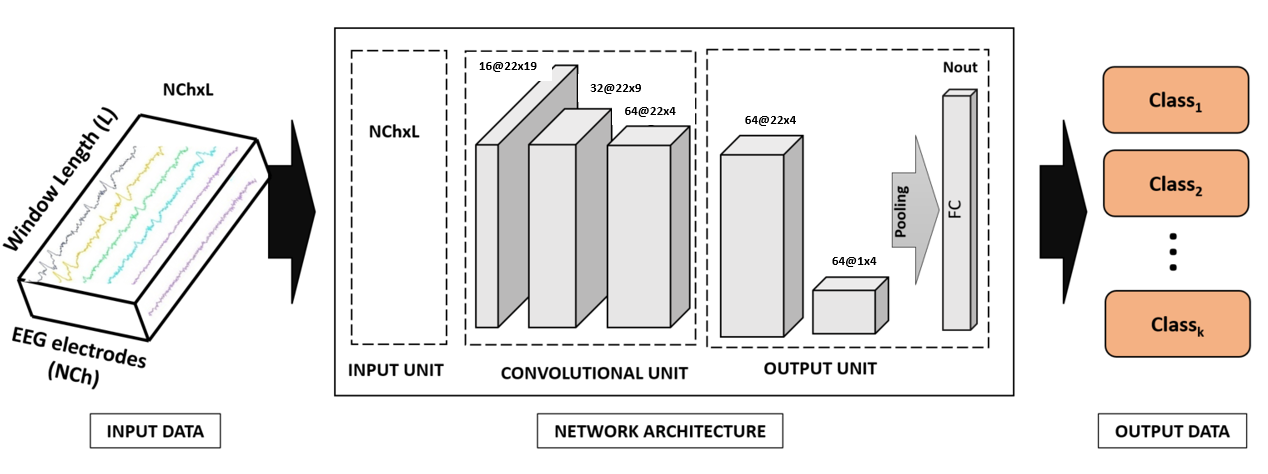
\includegraphics[width=0.5\textwidth]{img/FeatureProjectorModel CHM.png}
\end{figure}
\leavevmode\\
During the implementation of this procedure, a lot of problems of dependency on critical libraries has happened. Starting by cuda, for faster results it is used in all models, but it might not work if the architecture of the graphics card is too old. It is also not compatible with python 3.10 which was the version being worked on at the moment, it had to be switched to an environment with python 3.8 to avoid further issues.
\\